\chapter{Rigid Multibody Dynamics}
\label{chp:back_RBDynamics}

In this chapter, a mathematical groundwork for characterizing the dynamics of a floating-base multibody system is presented, setting a convention that is used throughout this work. Then, a first introduction to recursive algorithm for the computation of the dynamics of a multibody system is presented, in order to give a comprehensive understanding of the state of the art in the field of rigid multibody dynamics algorithms. In the forthcoming discussion, a 6D \textit{spatial vectors} notation firstly introduced by \citet{featherstone_rigid_2008} and successively integrated and adapted by \citet{traversaro_multibody_2019} is presented. This convention is adopted and will be used to describe the kinematics and dynamics of a floating-base multibody system in a unified manner.

\section{Formalisms and Notation}

\paragraph{Spatial Vectors} A spatial vector is a 6D vector that describes the motion of a rigid body in space.

In the case of a rigid body, the velocity of a point $P$ attached to the body respect to a reference frame attached to an arbitrary point $O$ in the space can be generally expressed by its angular component $\mathbf{\omega}$ about an axis passing through $O$ and its linear component $\mathbf{v} _P$, for which the following relation holds:

\begin{equation}
    v _P = \mathbf{\omega} \times \bar{OP}
\end{equation}

where $\bar{OP}$ is the position vector of $P$ with respect to $O$. This holds for any point $P$ on the rigid body. In order to simplify the notation, introducing a Cartesian coordinate frame $\mathcal{O} _{xyz}$, we can define a basis of 6 spatial vectors $\mathcal{D} _O = \{\mathbf{d} _i\} ^6 _{i=1}$ as:

\begin{equation}
    \mathcal{D} _O = \{ \mathbf{d} _{O _x}, \mathbf{d} _{O _y}, \mathbf{d} _{O _z}, \mathbf{d} _x, \mathbf{d} _y, \mathbf{d} _z \} \subset \mathcal{M} ^6
\end{equation}

where $\mathcal{M} ^6$ is the space of 6D vectors, defining a Pl\"ucker coordinate system on $\mathcal{M} ^6$ as shown in \cref{fig:pluecker}.

\begin{figure}
    \centering
    \caption{Pl\"ucker motion coordinate system}
    \label{fig:pluecker}
    \tikzset{every picture/.style={line width=0.75pt}}
    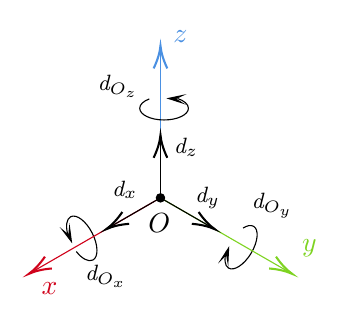
\begin{tikzpicture}[x=0.75pt,y=0.75pt,yscale=-1,xscale=1]
        \draw [color={rgb, 255:red, 74; green, 144; blue, 226 }  ,draw opacity=1 ]   (249.79,80.38) -- (249.79,9.08) ;
        \draw [shift={(249.79,7.08)}, rotate = 90] [color={rgb, 255:red, 74; green, 144; blue, 226 }  ,draw opacity=1 ][line width=0.75]    (10.93,-3.29) .. controls (6.95,-1.4) and (3.31,-0.3) .. (0,0) .. controls (3.31,0.3) and (6.95,1.4) .. (10.93,3.29)   ;
        \draw  [draw opacity=0] (257.99,32.5) .. controls (261.16,33.51) and (263.25,35.24) .. (263.25,37.21) .. controls (263.25,40.32) and (258,42.85) .. (251.52,42.85) .. controls (245.05,42.85) and (239.8,40.32) .. (239.8,37.21) .. controls (239.8,35.38) and (241.61,33.75) .. (244.41,32.72) -- (251.52,37.21) -- cycle ; \draw   (257.99,32.5) .. controls (261.16,33.51) and (263.25,35.24) .. (263.25,37.21) .. controls (263.25,40.32) and (258,42.85) .. (251.52,42.85) .. controls (245.05,42.85) and (239.8,40.32) .. (239.8,37.21) .. controls (239.8,35.38) and (241.61,33.75) .. (244.41,32.72) ;
        \draw  [draw opacity=0] (205.05,97.73) .. controls (204.06,93.79) and (204.55,90.48) .. (206.55,89.46) .. controls (209.33,88.05) and (213.96,91.58) .. (216.9,97.35) .. controls (219.84,103.12) and (219.97,108.94) .. (217.19,110.35) .. controls (215.09,111.42) and (211.93,109.66) .. (209.25,106.25) -- (211.87,99.91) -- cycle ; \draw   (205.05,97.73) .. controls (204.06,93.79) and (204.55,90.48) .. (206.55,89.46) .. controls (209.33,88.05) and (213.96,91.58) .. (216.9,97.35) .. controls (219.84,103.12) and (219.97,108.94) .. (217.19,110.35) .. controls (215.09,111.42) and (211.93,109.66) .. (209.25,106.25) ;
        \draw  [draw opacity=0] (289.6,94.92) .. controls (291.53,93.69) and (293.37,93.33) .. (294.68,94.12) .. controls (297.34,95.72) and (296.8,101.52) .. (293.45,107.07) .. controls (290.11,112.61) and (285.24,115.81) .. (282.57,114.2) .. controls (280.67,113.05) and (280.4,109.78) .. (281.61,105.98) -- (288.62,104.16) -- cycle ; \draw   (289.6,94.92) .. controls (291.53,93.69) and (293.37,93.33) .. (294.68,94.12) .. controls (297.34,95.72) and (296.8,101.52) .. (293.45,107.07) .. controls (290.11,112.61) and (285.24,115.81) .. (282.57,114.2) .. controls (280.67,113.05) and (280.4,109.78) .. (281.61,105.98) ;
        \draw  [fill={rgb, 255:red, 0; green, 0; blue, 0 }  ,fill opacity=1 ] (205.98,94.78) -- (206.86,101.37) -- (202.81,96.09) -- (205.63,98.4) -- cycle ;
        \draw  [fill={rgb, 255:red, 0; green, 0; blue, 0 }  ,fill opacity=1 ] (279.01,110.18) -- (282.61,104.59) -- (282.28,111.23) -- (281.63,107.65) -- cycle ;
        \draw  [fill={rgb, 255:red, 0; green, 0; blue, 0 }  ,fill opacity=1 ] (260,34.53) -- (253.67,32.48) -- (260.18,31.11) -- (256.88,32.65) -- cycle ;
        \draw [color={rgb, 255:red, 126; green, 211; blue, 33 }  ,draw opacity=1 ]   (249.79,80.38) -- (311.53,116.02) ;
        \draw [shift={(313.27,117.02)}, rotate = 210] [color={rgb, 255:red, 126; green, 211; blue, 33 }  ,draw opacity=1 ][line width=0.75]    (10.93,-3.29) .. controls (6.95,-1.4) and (3.31,-0.3) .. (0,0) .. controls (3.31,0.3) and (6.95,1.4) .. (10.93,3.29)   ;
        \draw [color={rgb, 255:red, 208; green, 2; blue, 27 }  ,draw opacity=1 ]   (249.79,80.37) -- (218.61,98.38) -- (188.04,116.02) ;
        \draw [shift={(186.31,117.02)}, rotate = 330] [color={rgb, 255:red, 208; green, 2; blue, 27 }  ,draw opacity=1 ][line width=0.75]    (10.93,-3.29) .. controls (6.95,-1.4) and (3.31,-0.3) .. (0,0) .. controls (3.31,0.3) and (6.95,1.4) .. (10.93,3.29)   ;
        \draw    (249.79,80.38) -- (249.79,52.13) ;
        \draw [shift={(249.79,50.13)}, rotate = 90] [color={rgb, 255:red, 0; green, 0; blue, 0 }  ][line width=0.75]    (10.93,-3.29) .. controls (6.95,-1.4) and (3.31,-0.3) .. (0,0) .. controls (3.31,0.3) and (6.95,1.4) .. (10.93,3.29)   ;
        \draw    (249.79,80.38) -- (274.25,94.5) ;
        \draw [shift={(275.99,95.5)}, rotate = 210] [color={rgb, 255:red, 0; green, 0; blue, 0 }  ][line width=0.75]    (10.93,-3.29) .. controls (6.95,-1.4) and (3.31,-0.3) .. (0,0) .. controls (3.31,0.3) and (6.95,1.4) .. (10.93,3.29)   ;
        \draw    (249.79,80.37) -- (225.32,94.5) ;
        \draw [shift={(223.59,95.5)}, rotate = 330] [color={rgb, 255:red, 0; green, 0; blue, 0 }  ][line width=0.75]    (10.93,-3.29) .. controls (6.95,-1.4) and (3.31,-0.3) .. (0,0) .. controls (3.31,0.3) and (6.95,1.4) .. (10.93,3.29)   ;
        \draw (191.23,119.9) node [anchor=north west][inner sep=0.75pt]  [color={rgb, 255:red, 208; green, 2; blue, 27 }  ,opacity=1 ]  {$x$};
        \draw (316.73,99.4) node [anchor=north west][inner sep=0.75pt]  [color={rgb, 255:red, 126; green, 211; blue, 33 }  ,opacity=1 ]  {$y$};
        \draw (254.73,-1.35) node [anchor=north west][inner sep=0.75pt]  [color={rgb, 255:red, 74; green, 144; blue, 226 }  ,opacity=1 ]  {$z$};
        \draw (212.25,111.65) node [anchor=north west][inner sep=0.75pt]  [font=\footnotesize]  {$\mathit{d}_{O_{x}}$};
        \draw (218.25,20.15) node [anchor=north west][inner sep=0.75pt]  [font=\footnotesize]  {$\mathit{d}_{O_{z}}$};
        \draw (292.5,76.9) node [anchor=north west][inner sep=0.75pt]  [font=\footnotesize]  {$\mathit{d}_{O_{y}}$};
        \draw (255,50.4) node [anchor=north west][inner sep=0.75pt]  [font=\footnotesize]  {$\mathit{d}_{z}$};
        \draw (225.25,70.9) node [anchor=north west][inner sep=0.75pt]  [font=\footnotesize]  {$\mathit{d}_{x}$};
        \draw (265.25,73.9) node [anchor=north west][inner sep=0.75pt]  [font=\footnotesize]  {$\mathit{d}_{y}$};
        \draw (242.75,86.65) node [anchor=north west][inner sep=0.75pt]    {$O$};
        \draw [fill={rgb, 255:red, 0; green, 0; blue, 0 }  ,fill opacity=1 ]  (249.79, 80.38) circle [x radius= 2, y radius= 2]   ;
    \end{tikzpicture}
\end{figure}

\dots

\paragraph{Spatial Velocity} \dots The spatial velocity of a rigid body is defined as:

\begin{equation}
    \mathbf{v} _P = \begin{bmatrix}
        \mathbf{v} _P \\
        \boldsymbol{\omega} _P
    \end{bmatrix}
\end{equation}

where $\mathbf{v} _P$ is the linear velocity of the point $P$ and $\boldsymbol{\omega} _P$ is the angular velocity of the body.

\paragraph{Spatial Forces} \dots The spatial force acting on a rigid body is defined as:

\begin{equation}
    \mathbf{f} = \begin{bmatrix}
        \mathbf{f} \\
        \boldsymbol{\tau}
    \end{bmatrix}
\end{equation}



\section{Problem Formalization}

Starting from the equation of motion of a robot manipulator:

\begin{equation}
    \mathbf{M}(q)\dot{\boldsymbol{\nu}} + \mathbf{h}(q,\boldsymbol{\nu}) = \mathbf{B}\boldsymbol{\tau} + \mathbf{J} ^T \mathbf{f}
\end{equation}

where:

\begin{itemize}
    \item $\mathbf{M}(q)$ is the inertia matrix
    \item $\mathbf{h}(q,\boldsymbol{\nu})$ is the Coriolis vector
    \item $\mathbf{B}$ is the actuation matrix
    \item $\boldsymbol{\tau}$ is actuation torques vector
    \item $\mathbf{J}$ is the Jacobian matrix
    \item $\mathbf{f}$ is the external forces vector
\end{itemize}

we can isolate the terms related to the base link (usually in position 0) from the joints' poses:

\begin{align}
    \boldsymbol{\nu} =
    \begin{bmatrix}
        \mathrm{\mathbf{v}} \\
        \dot{\mathbf{s}}
    \end{bmatrix} &  &
    \dot{\boldsymbol{\nu}} =
    \begin{bmatrix}
        \dot{\mathrm{\mathbf{v}}} \\
        \ddot{\mathbf{s}}
    \end{bmatrix}
\end{align}

where $\mathrm{\mathbf{v}} \in \mathbb{R} ^{6}$ and $\mathbf{s} \in \mathbb{R}^{N_B}$, we get to the form:

\begin{equation}
    \begin{bmatrix}
        \mathbf{M} _{\mathcal{B}}(q)     & \mathbf{M} _{\mathcal{B}S}(q) \\
        \mathbf{M} _{\mathcal{B}S} ^T(q) & \mathbf{M} _s(q)
    \end{bmatrix}
    \begin{bmatrix}
        \dot{\mathrm{\mathbf{v}}} \\
        \ddot{\mathbf{s}}
    \end{bmatrix}+
    \begin{bmatrix}
        \mathbf{h} _{\mathcal{B}} \\
        \mathbf{h} _S
    \end{bmatrix}=
    \begin{bmatrix}
        \mathbb{0} \\
        \mathbb{1}
    \end{bmatrix}
    \boldsymbol{\tau}
    +
    \begin{bmatrix}
        \mathbf{J} _{\mathcal{B}} \\
        \mathbf{J} _S
    \end{bmatrix} ^T
    \mathbf{f}
\end{equation}

Given that the dynamics of the set of motors can be described by the following equation:

\begin{equation}
    \label{eqn:mot_dyn}
    \mathbf{I} _R \ddot{\boldsymbol{\theta}} + \mathbf{K}_v \dot{\boldsymbol{\theta}} = \boldsymbol{\tau}_m
\end{equation}

where $\mathbf{K _v}$ is the diagonal matrix of motor viscous coefficients and $\mathbf{I}_R$ is the diagonal matrix of motors' inertias. Considering that given the set of transmission ratios $\boldsymbol{\Gamma}$, the relation between the joints' velocities and the motors' velocities is:

\begin{align}
    \mathbf{s} = \boldsymbol{\theta} \boldsymbol{\Gamma} &  & \dot{\mathbf{s}} = \dot{\boldsymbol{\theta}} \boldsymbol{\Gamma} &  & \ddot{\mathbf{s}} = \ddot{\boldsymbol{\theta}} \boldsymbol{\Gamma}
\end{align}

we can rewrite the equation \ref{eqn:mot_dyn} in the joints' space as:

\begin{equation}
    \label{eqn:mot_dyn_jointspace}
    \boldsymbol{\tau} = \boldsymbol{\Gamma} ^{-T} (\mathbf{I} _R\boldsymbol{\Gamma} ^{-1} \ddot{s} + \mathbf{K}_v \boldsymbol{\Gamma} ^{-1}\dot{s})
\end{equation}

Therefore, the \ac{EoM} of the multibody system can be rewritten as:

\begin{equation}
    \underbrace{\begin{bmatrix}
            \mathbf{M} _{\mathcal{B}}(q)     & \mathbf{M} _{\mathcal{B}S}(q)                                                      \\
            \mathbf{M} _{\mathcal{B}S} ^T(q) & \mathbf{M} _s(q) + \boldsymbol{\Gamma} ^{-T}\mathbf{I} _R\boldsymbol{\Gamma} ^{-1}
        \end{bmatrix}} _{\mathbf{\bar{M}}(q)}
    \begin{bmatrix}
        \dot{\mathrm{\mathbf{v}}} \\
        \ddot{\mathbf{s}}
    \end{bmatrix}+
    \mathbf{h}
    (q,\boldsymbol{\nu}) =
    \underbrace{\begin{bmatrix}
            \mathbb{0} \\
            \boldsymbol{\Gamma} ^{-T}
        \end{bmatrix}} _{\mathbf{\bar{B}}}
    \boldsymbol{\tau} _m
    +
    \mathbf{J} ^T
    \mathbf{f}
    -
    \underbrace{\begin{bmatrix}
            \mathbb{0} \\
            \boldsymbol{\Gamma} ^{-T}\mathbf{K _v}\boldsymbol{\Gamma} ^{-1}
        \end{bmatrix}} _\mathbf{\bar{K _v}}
    \begin{bmatrix}
        \mathrm{\mathbf{v}} \\
        \dot{\mathbf{s}}
    \end{bmatrix}
\end{equation}

or, in a more compact form that will be used for computation as:

\begin{equation}
    \mathbf{\bar{M}}(q)\dot{\boldsymbol{\nu}} + \mathbf{h}(q,\boldsymbol{\nu}) = \mathbf{\bar{B}}\boldsymbol{\tau} _m + \mathbf{J} ^T \mathbf{f} - \bar{\mathbf{K _v}}\boldsymbol{\nu}
\end{equation}

